\documentclass[12pt]{article}
\usepackage[utf8]{inputenc}
\usepackage{amssymb,amsmath}
\usepackage{hyperref}
\usepackage{graphicx}
\author{Sven-Hendrik Haase, Ingo Eibes, Alexander Bufe,\\Benjamin Wegner, Elena Noll}
\title{GDB HA zum 8.11.12}
\date{\today}
\begin{document}
\setcounter{secnumdepth}{0}
\maketitle

\section{Aufgabe 1}
\subsection{a)}
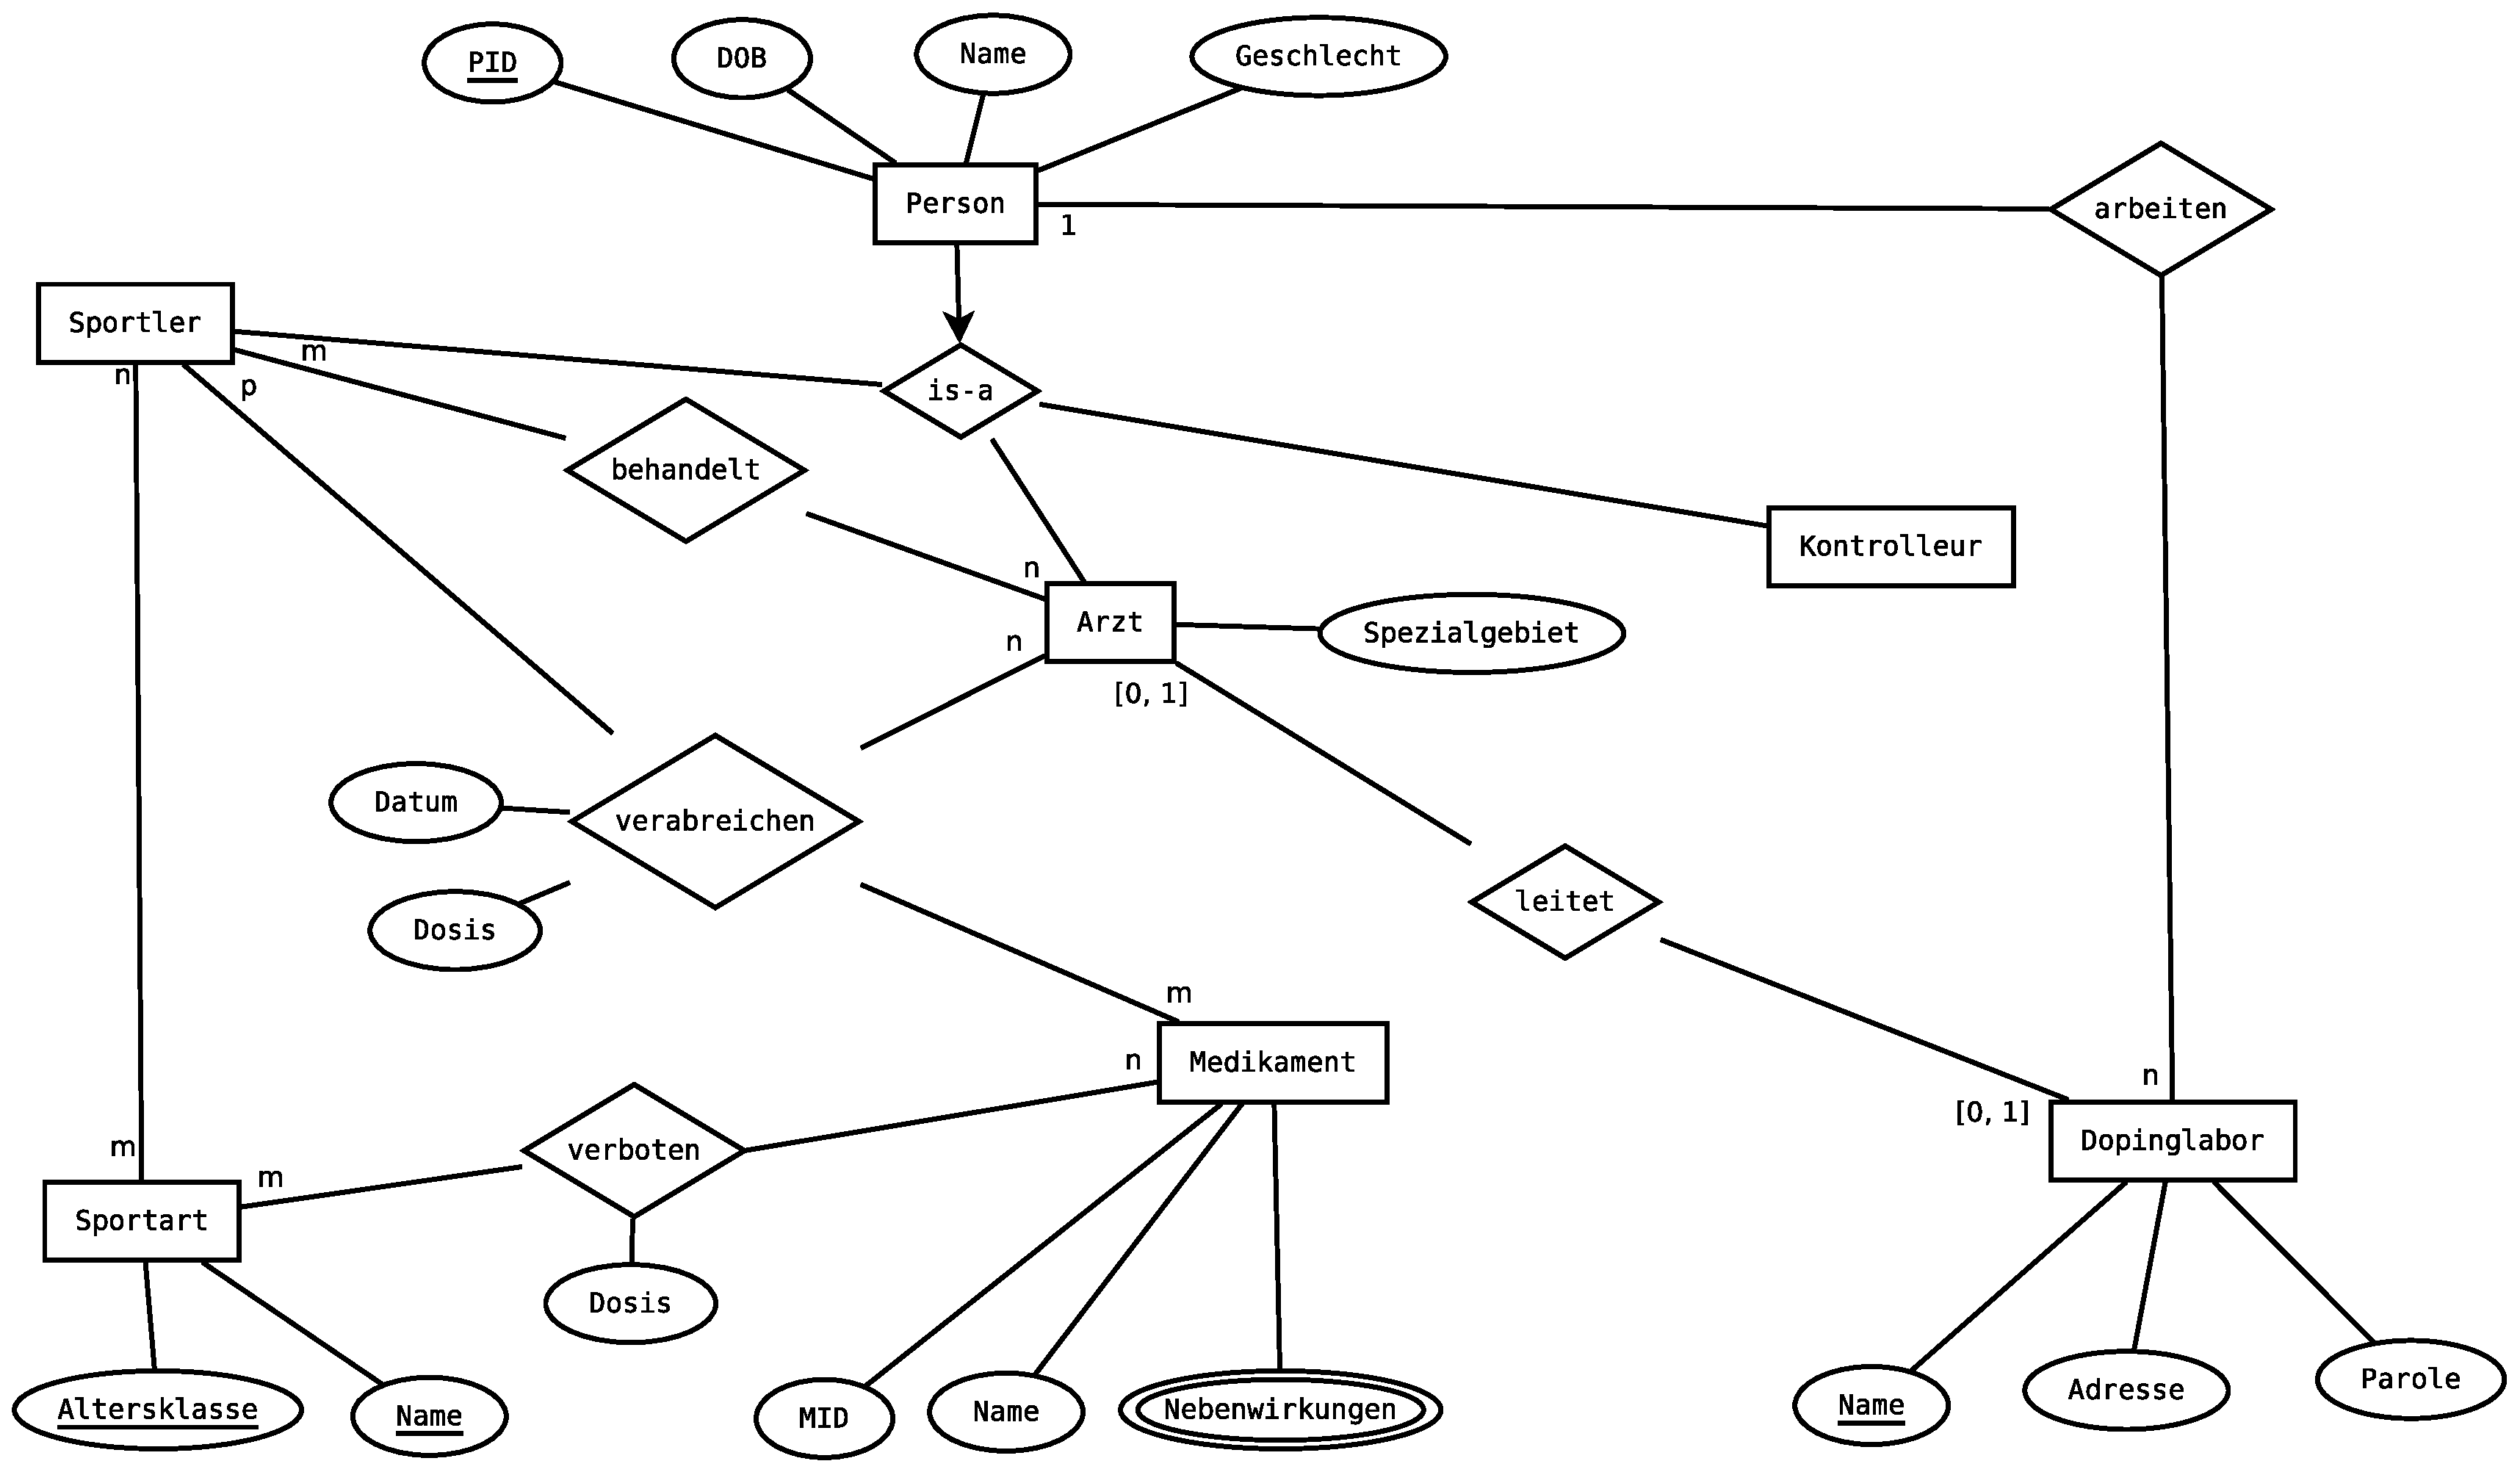
\includegraphics[scale=0.25]{Aufgabe2.eps}

\newpage
\subsection{b)}
\begin{enumerate}
\item Nur für bestimmte Sportarten dürfen bestimmte Medikamente verabreicht werden.
\item Bestimmte Sportler dürfen bestimmte Medikamente nicht nehmen (z.B. wegen Krankheit oder Allergie)
\end{enumerate}

\section{Aufgabe 2}
\subsection{a)}
Ein Fahrzeug besteht aus einem eindeutigen KFZ-Kennzeichen (als KFZ bezeichnet) und aus einem Fahrzeugtyp.
Eine Person besteht aus einer eindeutigen Servicenummer (als SVNr bezeichnet) und aus einem Namen.
Ein Fahrzeug kann genau auf eine Person gemeldet sein. Auf eine Person können mehrere Fahrzeuge gemeldet sein.

\subsection{b)}
Eine Vorlesung ist durch eine eindeutige Vorlesungsnummer (als VNr bezeichnet) und einen Namen definiert.
Zu einer Vorlesung kann es 0 bis 5 Nachfolger geben, die auf die Vorlesung aufbauen.
Zu einer Vorlesung kann es 0 bis n Vorgänger geben, auf die die Vorlesung aufbaut.

\subsection{c)}
Eine Person besteht aus einem Vornamen und einem Nachnamen, die beiden Attribute zusammen legen den Key fest. Zudem hat eine Person noch ein Adressen-Attribut.
Ein Mann hat ein Paar Schuhe und ist eine Person.
Eine Frau hat mehrere Paare Schuhe und ist ebenfalls eine Person

\subsection{d)}
Ein Superheld hat eine eindeutige HNr als Key, einen Namen und ein Einsatzgebiet.
Eine Superkraft wird durch eine Beschreibung und eine eindeutige Bezeichnung festgelegt.
Mehrere Superhelden können mehrere Superkräfte haben, die von einer Einschränkung gekennzeichnet ist.

\subsection{e)}
Ein Professor hat eine eindeutige ProfNr und einen Namen.
Ein Modul hat eine eindeutige MNr und einen Titel.
Ein Prüfling hat eine eindeutige MNr, einen Namen und einen Studiengang.
In einem Modul können 0 bis n Prüflinge eine Prüfung ablegen. Ein Professor kann 0 – k Prüflinge prüfen. Ein Prüfling kann in 0 – 20 Modulen von 0 - 20 Professoren eine Prüfung ablegen. Dabei ist eine Prüfung immer von einem Datum und einer Note festgelegt.

\section{Aufgabe 3}
\subsection{a)}
Betrachtet man nur die 6 aufgelisteten Entitäten und geht davon aus, dass keine weiteren hinzukommen, könnte man die Attribute Vorname, Geb.-Dat. und Telefonnr. als Key verwenden, da diese in allen 6 Entitäten mit verschiedenen Werten belegt sind. Sie gewährleisten also die Eindeutigkeit und sind zudem die optimale Lösung in Bezug darauf, dass es minimal ist. Oft wird die Kombination aus Vorname und Nachname als Key verwendet. Dies wäre in unserem Fall aber keine optimale Lösung, da man einen Key wie oben beschrieben auch aus einem Attribut wählen kann.

\subsection{b)}
Da man aber davon ausgehen muss, dass weitere Entitäten hinzukommen und es nicht ausgeschlossen ist, dass 2 oder mehrere Personen den selben Vornamen, das selbe Geb.-Dat. oder die selbe Telefonnr. haben, kann man keinen Key aus einem Attribut wählen. Auch mit 2 Attributen, die kombiniert werden, wird es schwierig. Es gibt durchaus Personen mit den selben Vor- und Nachnamen, Personen, die die selbe Fächerkombination belegt haben oder die im selben Ort wohnen und am gleichen Tag geboren wurden. Eine eventuell mögliche Kombination aus 2 Attributen wäre aber der Vorname mit der Telefonnummer. Es kommt eher selten vor, dass 2 Personen mit dem selben Vornamen im gleichen Haus oder der gleichen Wohnung wohnen. Kombinationen aus 3 Attributen könnten ebenfalls in Frage kommen. Die 3 Attribute Vorname, Nachname, und Geburtsdatum zu kombinieren, wäre eine Möglichkeit. Es ist zwar immer noch nicht zu 100\% ausgeschlossen, dass es nicht 2 Personen mit dem selben Vor - und Nachnamen gibt und diese am selben Tag Geburtstag haben, aber die Wahrscheinlichkeit, dass dies vorkommt, ist sehr gering. Eine Lösung einen wirklich eindeutigen und minimalen Key zu wählen, ist indem man ein zusätzliches Attribut (z.B. ID oder Index) hinzunimmt, welches unique ist und mit einem auto-increment automatisch erhöht wird.  So hätte man einen minimalen und wirklich eindeutigen Key zur Identifikation.
\end{document}
